% REVISÃO DE LITERATURA--------------------------------------------------------

\chapter{REVISÃO DE LITERATURA}
\label{chap:fundamentacao-teorica}

Neste capítulo será descrito o referencial teórico que embasou esta pesquisa. Descrevendo a relação entre games e educação; comentando sobre jogos de plataforma \textit{2D} e jogos no ensino de História. Também apresentando três trabalhos correlatos (artigos publicados no SBGames) que apresentam jogos educativos para o ensino de História.

\section{Games e Educação}
\label{sec:gameseeducacao}

Com o aumento exponencial do uso de tecnologia em todas as idades, o acesso a informações se tornou muito fácil, surgiram novas formas de agir e pensar. Um profissional capaz de se reinventar de acordo com as necessidades do momento se tornou mais desejado do que um profissional que sempre age da mesma forma, que nunca está disposto a mudar. Essa nova dinâmica do mercado fez com que o modelo de ensino das escolas fosse questionado, pois aquele padrão onde o professor simplesmente transmite as informações e os alunos as decoram ficou defasado e desmotivador. Agora é necessário que os alunos aprendam a aprender, que sejam capazes de construir novos conhecimentos a partir das informações disponíveis \cite{bib:medeiros2012}.

Um jogo pode ser definido como ``um sistema no qual os jogadores se envolvem em um conflito artificial, definido por regras, que implica um resultado quantificável"\space\cite{bib:salen2012}. Já os jogos educacionais são aqueles criados para ensinar com diversão. São desenvolvidos para fins pedagógicos e geralmente contam com as crianças como público alvo. Contudo, todos os tipos de jogos permitem a obtenção de conhecimentos do mundo real pelos jogadores e muitos jogos eletrônicos são educativos por ``acidente"\space\cite{bib:novak2010}.

\citeonline{bib:medeiros2012} encorajam o uso de jogos na educação, afirmando que, além de serem fontes de diversão, os jogos podem ser utilizados para vários fins educativos e como instrumentos de desenvolvimento de crianças e jovens. Os autores explicam que, para as crianças, o jogo constitui um fim, onde o objetivo principal é a diversão. Já para os educadores, o jogo é um meio, um veículo que permite transmitir uma mensagem educativa de forma atraente e prazerosa, cabe ao professor escolher o jogo que melhor se aplica ao conteúdo que deseja ensinar.

Com o desenvolvimento tecnológico, surgiu uma nova modalidade de jogos, os eletrônicos, mas a utilização desse tipo de jogo na área da educação ainda sofre preconceitos, pois muitas vezes ele é visto como uma perda de tempo, algo que os jovens acabam se viciando e que não os ensina nada \cite{bib:medeiros2012}.

Jogos eletrônicos educacionais atuam diretamente na necessidade de romper com o atual paradigma da educação, levando-se em consideração: A importância da interatividade para manter a atenção do estudante; o desenvolvimento de um ambiente sem riscos no qual o aluno possa testar os seus conhecimentos; e a individualidade de cada aprendiz, uma vez que cada um pode aprender de forma diferenciada, assimilando conhecimentos e experiências em seu próprio ritmo \cite{bib:medeiros2012}.

\section{Jogos de Plataforma \textit{2D}}
\label{sec:plataforma2D}

Na década de $1980$ surgiram os primeiros jogos plataforma de ação e aventura, \textit{Donkey Kong}\footnote{\url{http://pt-br.donkey-kong-country.wikia.com/wiki/Donkey\_Kong(personagem)}} e \textit{Mario}\footnote{\url{http://desciclopedia.org/wiki/Mario\_(personagem)}} eram personagens que apresentavam mecânicas de interação em duas dimensões \textit{(2D)}. Os jogadores podiam andar para a direita, esquerda e para baixo e executar ações de pular, subir em escadas e atacar. Já nos anos $90$, com o desenvolvimento das tecnologias de computação, surgiram os jogos em três dimensões \textit{(3D)}. \textit{Wolfenstein 3D}\footnote{\url{http://wolf3d.atw.hu/}} e \textit{Doom}\footnote{\url{desciclopedia.org/wiki/Doom}} revolucionaram a história dos videogames por serem os primeiros jogos do gênero de tiro em primeira pessoa que apresentaram uma movimentação tridimensional semelhante ao mundo real, davam cinco graus de liberdade aos jogadores e tinham texturas consideradas realistas para a época, mas exigiam mais poder de processamento dos computadores ou videogames \cite{bib:lopes2016}.

Considerando os avanços da indústria dos jogos digitais e das tecnologias computacionais, pode-se afirmar que consoles, videogames portáteis, computadores, \textit{smartphones} e \textit{tablets} da atualidade são capazes de processar jogos com gráficos \textit{3D}. Desta forma, escolher entre fazer um jogo \textit{2D} ou \textit{3D} é de responsabilidade dos \textit{designers} de jogos e a escolha é feita através de suas propostas de jogabilidade e da preferência do seu público alvo pelo estilo de jogo.

No decorrer dos anos as desenvolvedoras adaptaram suas franquias de acordo com a melhoria das tecnologias. Jogos que surgiram na época do \textit{2D} como \textit{Prince of Persia}\footnote{\url{https://classicreload.com/prince-of-persia.html}}, \textit{Super Mario} e \textit{Castlevania}\footnote{\url{castlevania.wikia.com/wiki/Games}}, acompanharam a evolução e ganharam versões tridimensionais. Em contraponto, algumas franquias da atualidade que surgiram na era tridimensional como \textit{Assassin’s Creed}\footnote{\url{https://www.ubisoft.com/en-gb/game/assassins-creed}} e \textit{Mirro's Edge}\footnote{\url{www.mirrorsedge.com/pt\_BR/}} tomaram o caminho inverso e criaram versões com duas dimensões. Com características e interações parecidas, mas com diferenças de jogabilidade por causa das três ou duas dimensões, nem todos os jogos das franquias citadas acima agradaram $100\%$ dos fãs. Estudar as percepções dos usuários sobre executar interações em jogos com mecânicas \textit{2D} e \textit{3D} permite que sejam identificados os pontos específicos de interesse dos jogadores, os problemas que dificultam a execução das interações em cada modo de jogo e o equilíbrio necessário entre a diversão e o desafio \cite{bib:lopes2016}.

\section{Jogos no Ensino de História}
\label{sec:gameshistoria}

A História tem sido há alguns anos a fonte que retroalimenta os enredos de peças teatrais, obras literárias, filmes, novelas, histórias em quadrinhos, animes, games etc. Essa parceria no caso do cinema, data mais de um século e, até hoje, alguns títulos considerados clássicos são indicados ou exibidos nas salas de aula para promover aprendizagens, como exemplo: Danton: o processo da revolução $(1982)$, O Nome da Rosa $(1986)$, $1492$ -- A Conquista do Paraíso $(1992)$, A lista de \textit{Schindler} $(1993)$, dentre outros. Já na mídia televisiva brasileira o resultado da aproximação com a História ficou conhecido como ``trabalhos de época", aparecendo apenas na década de $70$, lançando sucessos de audiência conhecidos nacionalmente e, em alguns casos, internacionalmente tais como: Escrava Isaura $(1970)$, Sinhá Moça $(1986)$ e etc \cite{bib:neves2012}.

O uso da História pelos jogos digitais seguiu o mesmo caminho dessas duas mídias, aliando conteúdos históricos e ficção o que possibilitava não apenas a visualização, mas também a interação, ou até mesmo, a imersão nos ambientes simulados. Cabe aqui ressaltar, que, antes mesmo de ser utilizada nos jogos com formato digital, a História já era utilizada como fonte dos jogos no formato ``analógico"\space(conhecidos também como jogos de tabuleiro). Destacam-se, entre esses jogos: \textit{War} $(1972)$, \textit{Yatzi} $(1983)$, Cabral: descobrimento e criação $(2000)$, Alexander $(2003)$, \textit{Age of Heroes} $(2003)$, \textit{Angus} -- Batalhas Medievais $(2004)$, \textit{Band of Heroes} $(2005)$, Conquistadores $(2006)$, \textit{War} Império Romano $(2007)$ dentre outros \cite{bib:neves2012}.

Os acontecimentos e fatos históricos tiveram suas primeiras aparições nos jogos digitais do tipo \textit{Role-Playing Game (RPG)}, que começaram a surgir durante a década de $1970$. Estes jogos contribuíram expressivamente para a compreensão de que a História poderia ser utilizada nesses suportes, assim como já acontecia em outras mídias. Tais jogos deram sua parcela de ajuda, na medida em que articulavam em seus enredos jornadas épicas para enriquecer suas narrativas (sem um caminho linear ou final pré-estabelecido) com personagens e ambientes que remetiam o jogador ao passado e a um mundo de fantasia. Dessa forma, ao incorporar narrativas, os jogos digitais transformaram a tradição narrativa visual e revolucionaram a forma como as histórias passaram a ser contadas \cite{bib:novak2010}.

A partir daí, a História marcava presença nos jogos digitais de estratégia, que, por sua vez, adotavam em seu enredo acontecimentos históricos reportando épocas passadas, como temática central ou apenas pano de fundo para construção do enredo, mesclando ficção aos fatos ``reais". Os primeiros jogos de estratégia geralmente se desenrolavam em ambiente militar, no qual o jogador tinha que gerir os recursos e a construção de diversos tipos de edifícios e unidades \cite{bib:neves2012}.

O desenvolvimento dos jogos de ficção histórica resulta de adaptações, montagens, restrições, seleções, generalizações e, até mesmo, criações espontâneas e falsificadas, que, às vezes, não guarda quaisquer relações com os acontecimentos ditos ``reais"\space -- tornando-se, assim, uma ``história de mentira"\space \cite{bib:neves2012}. Nessa lógica, simulam acontecimentos e fatos que se produzem nas e sobre as variadas dimensões da vida, no tempo e no espaço, como uma determinada sociedade, política, economia, cultura que pode ser realista ou alegórica, fidedigna ou fantasiosa, linear ou fragmentada.

Os games de História simulam e não somente representam os fatos ou acontecimentos históricos -- como fazem os artistas plásticos em suas telas, os dramaturgos em suas peças ou os cineastas em seus filmes. Esses jogos possibilitam ao jogador assumir o centro das decisões de um ambiente intencionalmente projetado com elementos históricos cuja finalidade é recriar e fazer alusão a um contexto histórico que, não mais pode ser vivenciado (no sentido do interator tomar decisões) senão por meio da simulação \cite{bib:neves2012}. Dito de outra forma, por meio do processo de imitação do mundo ``real", no qual é possível interagir, vivência a História do ponto de vista interno e não só externo -- como acontece nas representações -- através da tomada de diversas decisões: ir ou voltar, pegar itens ou descartá-los, atirar ou ignorar, invadir ou preservar etc.

\section{Trabalhos Correlatos}
\label{sec:correlatos}

Esta seção descreve três jogos que resultaram em publicações no SBGames $2016$ e que têm como objetivo principal a utilização como ferramenta para auxiliar no processo de ensino-aprendizagem de História.

\addtocontents{toc}{\protect\setcounter{tocdepth}{1}}
\subsection{Game Marabá -- Uma Viagem no Tempo} 

É um jogo \textit{RPG} aventura que tem como objetivo principal o aprendizado lúdico da história da fundação da cidade de Marabá-PA, através das aventuras de Velho Chico, espírito de Francisco Coelho da Silva (fundador de Marabá), que viaja no tempo do ano de $1906$ ao ano de $2015$, com a missão principal de reflorestar áreas do bairro Francisco Coelho (local de fundação da cidade) com árvores de caucho, e de construir uma nova ``Casa Marabá".

Para alcançar sua missão principal, Velho Chico tem como desafios lutar contra os esqueletos dos caucheiros, e dos guerreiros indígenas (figura \ref{fig:game-maraba}). E para enfrentar as batalhas irá contar com bônus de vidas, adquiridos através de comidas típicas da região. O jogador ``aprende"\space por meio de bônus de informações (caixas de diálogo com informações sobre a história da fundação de Marabá-PA), que são concedidos ao mesmo ao longo da sua evolução nas missões do game \cite{bib:teixeira2016}.

\begin{figure}[H]
	\centering
	\caption{Velho Chico enfrentando os inimigos -- caucheiros e indígenas, respectivamente}
	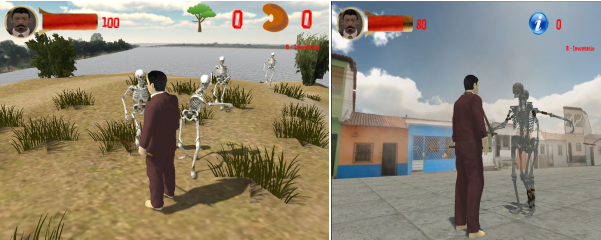
\includegraphics[width=0.9\textwidth]{figuras/game_maraba.png}
	\label{fig:game-maraba}
	{\fonte{\citeonline{bib:teixeira2016}}}
\end{figure}

\addtocontents{toc}{\protect\setcounter{tocdepth}{1}}
\subsection{Brasil Ball -- A Jornada}

É um jogo de plataforma \textit{2D} desenvolvido com o intuito de apresentar épocas importantes da história do Brasil, ou seja, cada fase do jogo corresponde a um evento histórico importante do país. Além disso, o jogo tem a missão de despertar um interesse maior na disciplina de História.

A primeira fase do jogo consiste no prólogo, em que o personagem Portugal conta a conquista da cidade de Ceuta em $1415$ e se inicia o império português, ilustrada na figura \ref{fig:brasil-ball}. A segunda fase consiste na luta de Portugal contra os índios, durante a invasão portuguesa ao território hoje pertencente ao Brasil. A terceira fase envolve os colonizadores portugueses em algumas das várias guerras pelo controle do Brasil contra holandeses e franceses. A quarta fase se passa durante as guerras de secessão que ocorreram durante o Brasil regência. A quinta fase ocorre na guerra do Paraguai, enquanto a sexta fase durante a guerra de Canudos. Por fim, a sétima fase ocorre durante a resistência armada à Ditadura \cite{bib:bb2016}.

\begin{figure}[H]
	\centering
	\caption{Cenário da primeira fase -- a conquista da cidade de Ceuta}
	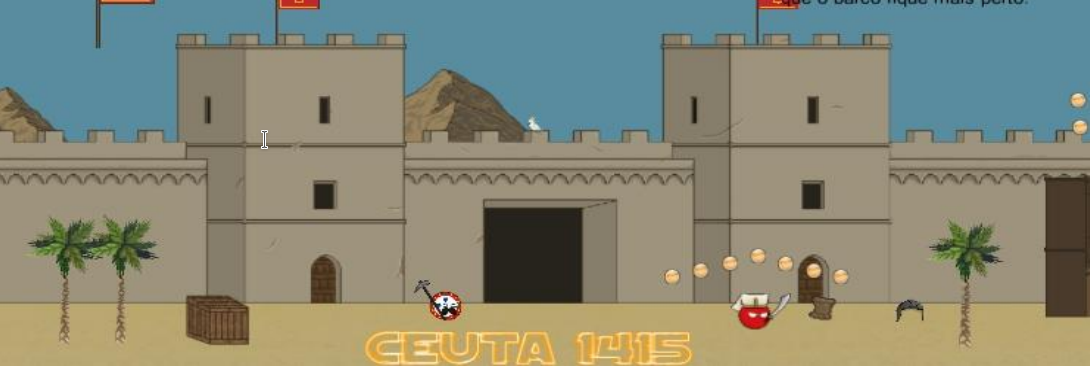
\includegraphics[width=0.9\textwidth]{figuras/brasil_ball.png}
	\label{fig:brasil-ball}
	{\fonte{\citeonline{bib:bb2016}}}
\end{figure}

\addtocontents{toc}{\protect\setcounter{tocdepth}{1}}
\subsection{Sete Povos -- \textit{mobile}}

É um jogo \textit{2D} que conta a história das missões jesuítas no Brasil, por meio da representação das rotinas diária das reduções (missões) jesuíticas, sendo desenvolvido para as plataformas \textit{Android} e \textit{iOS}. O jogador, ao acessar o menu principal, consegue visualizar toda a área de toda redução. Como apresentado na figura \ref{fig:sete-povos1}. Cada área representa uma atividade, como por exemplo construir empreendimentos ou cuidar do gado. O jogador pode escolher uma das atividades e então é direcionado para o jogo especifico para tal atividade.

Ao escolher uma região específica da redução para explorar, o jogador é direcionado para o jogo especifico e pode escolher entre: tutorial, aprender sobre questões históricas da temática envolvida ou iniciar o jogo. Os tutoriais, bem como a explicação histórica é apresentada por um personagem índio. Resultados do jogo \textit{mobile} são apresentados na figura \ref{fig:sete-povos2} onde é possível observar momentos de instrução e consulta histórica, além da tela de jogo \cite{bib:cassol2016}.

\begin{figure}[H]
	\centering
	\caption{Interface de apresentação do Jogo Sete Povos: O índio-jogador, pode escolher entre as diversas atividades realizadas do dia-a-dia da redução jesuítica}
	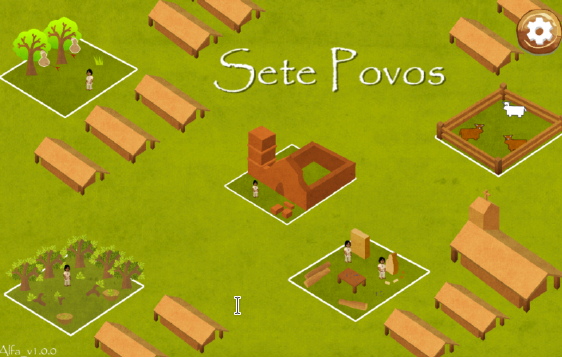
\includegraphics[width=0.53\textwidth]{figuras/sete_povos1.png}
	\label{fig:sete-povos1}
	{\fonte{\citeonline{bib:cassol2016}}}
\end{figure}

\begin{figure}[H]
	\centering
	\caption{Um índio instrui (esquerda) o jogador no tutorial e também explica a temática histórica reproduzida no jogo (direita).}
	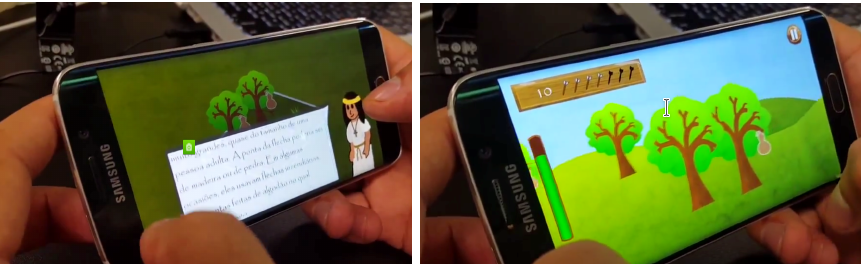
\includegraphics[width=.92\textwidth]{figuras/sete_povos2.png}
	\label{fig:sete-povos2}
	{\fonte{\citeonline{bib:cassol2016}}}
\end{figure}